%\label{Simple_Rainfall_HMM}
We begin testing HMMs for rainfall by developing a simple HMM that we can fit using only Baum Welch. We then simulate using our model and analyse its similarities to the observation data.

\section{Baum-Welch}
\label{Simple_Rainfall_HMM:Baum_Welch}
The only thing separating Grando's rainfall model from a simple HMM is the lack of an observation matrix \ref{Hidden_Markov:Definition}. In this section, we build this simpler model and then discuss finding the global optimum.

    \subsection{Building the Observation Matrix}
    \label{Simple_Rainfall_HMM:Baum_Welch:Building_the_Observation_Matrix}

    To use Baum-Welch, we require an observation probability matrix; thus, to use it, we must create one. To create a finite matrix of probabilities, we require our data to split into finite groups. Fortunately, the algorithm increases in computation cost linearly with the dimensions of the observation matrix rather than square compared to the number of states. Through efficient implementation, working with large observation matrices is feasible.

    Through looking at the datasets, we can see the maximum rainfall is usually up to 1000mm. In our case, this value was 743. Furthermore, the maximum precision of our data is integers. Thus, we can discretise our observations into integers up to the maximum rainfall for the given dataset. As we know from \ref{Hidden_Markov:Definition}, the rows of the observation matrix represent the states, and the columns represent the observations, giving us a matrix 3 by M matrix, where M is the number of observations.

    We can now apply Baum-Welch to produce a HMM model that simulates integer values of daily rainfall in mm up to a given maximum amount. Code files can be found in the "Baum Welch" folder under "MyCode". 

    \begin{note}
        The values of the alpha and beta helper functions become extremely small for a large sequence of observations. After about 1500 observations, these values become too precise to store in "long double" in our testing. This mathematically holds as the sum of the final alphas and betas represents the probability of observing the sequence \ref{Hidden_Markov:Evaluation:Forward_Backward_Algorithm:Alpha}, with a larger sequence, the probability naturally decreases. We avoid this problem by using a sequence of 1000 observations. 
        
        Using this method, one must ensure the alpha and beta values are not all being stored as zeros.
    \end{note}


    \subsection{Local vs Global Optimum}
    \label{Simple_Rainfall_HMM:Baum_Welch:Local_vs_Global_Optimum}


    Once again, from \ref{Hidden_Markov:Learning:Baum_Welch}, we know that Baum-Welch converges to local optima. This suggests there may be a superior optimum, a superior fit for the model, that we have not found. To ensure a satisfactory fit is found, we repeat the algorithm for multiple random starts, random initial distribution, transition matrix and observation matrix. While this does not guarantee we will find the global optima, it reassures us that our given optimum is reasonably suitable. 


    We choose to make three attempts. This choice was arbitrary. We recommend using a much larger number as we have selected this for simplicity of demonstration.

\section{Analysis}
\label{Simple_Rainfall_HMM:Analysis}
The program "BaumWelch" requires the data split into months in CSV files. For each month, it outputs the fitted transition matrix, observation matrix, initial vector, a Convergence log and a simulation using the model. This computation is done over 12 threads, allocating one for each month. For our data, we computed 100000 iterations of Baum-Welch. The three attempts took 1074.76, 1081.38 and 1076.16 seconds, respectively. In this section, we will graphically analyse our results.

    \subsection{Convergence}
    \label{Simple_Rainfall_HMM:Analysis:Convergence}

    We introduced a Convergence log to ensure the algorithm did Converge. The difference between the current and previous transition matrix, observation matrix, and initial distribution parameters was summed at each iteration. This sum represents the residual, which we expect to tend to 0 as the number of iterations tends to $\infty$.

    \begin{figure}
        \begin{subfigure}{.45\textwidth}
        \centering
        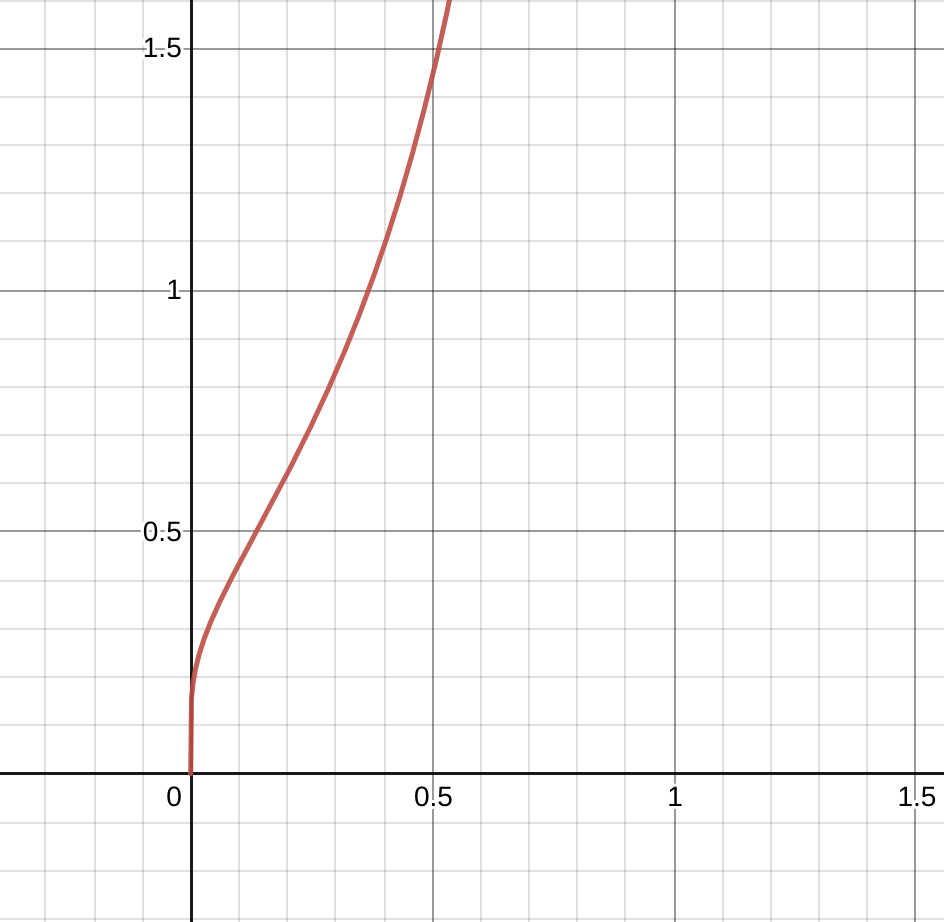
\includegraphics[width=\linewidth]{HMM_Only/function.png}
        \caption{Graph of the function $ y = \dfrac{-1}{ln(x)}$}
        \label{func}
        \end{subfigure}
        \begin{subfigure}{.45\textwidth}
        \centering
        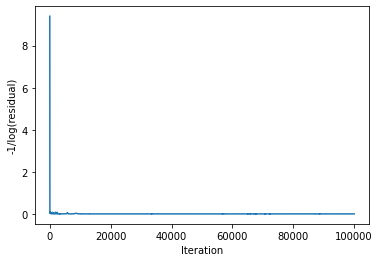
\includegraphics[width=\linewidth]{HMM_Only/convLog.png}
        \caption{Graph of function applied to residual of Baum-Welch against iteration number}
        \label{convlog}
        \end{subfigure}
        \caption{}
    \end{figure}

    The values decrease quite rapidly, thus to create a visual representation, we used the function $ y = \dfrac{-1}{ln(x)}$, where $x$ is the residual, to scale the values. We can see in Figure \ref{func} that our function is strictly increasing thus can be used for scaling. 

    Along with the CSV files containing the log, a graphical representation can be found in the Analysis Jupyter notebooks within each months folder. Figure \ref{convlog} shows one such graphical representation for the convergence log of attempt 1 for month 0. We can see that the residual converges to 0 relatively quickly, suggesting we could reduce the number of iterations. The convergence itself confirms that our two matrices and our initial distribution contain values close to the local optima. 

    \subsection{Selecting an Optimum}
    \label{Simple_Rainfall_HMM:Analysis:Selecting_an_Optimum}

    As mentioned earlier, we perform multiple random starts to try and obtain the global optimum. However, we do not know if it is the "most optimum" from the model alone. To do this, we count frequencies. 

    For each attempt, we count and record the frequency of occurrence of each integer in our observation set from our training rainfall data of 1000 observations as well as from our simulation generated by the HMM, also containing 1000 observations. We now find the difference between the two sets of frequencies, square the given value and then take a sum. The attempt the lowest sum of squares is then accepted as the most optimum optima. 

    For our example of month 0, we had the following results:
    \begin{center}
    \begin{tabular}{c | c}
        Attempt & Sum of Square difference \\
        \hline
        1 & 656 \\
        2 & 672 \\
        3 & 1692
    \end{tabular}
    \end{center}

    As such, we selected attempt 1 for our testing. The attempt selected for each month is in the below table.

    \begin{center}
    \begin{tabular}{c | c | c | c | c | c | c | c | c | c | c | c | c}
        Month   &  0  & 1 & 2 & 3 & 4 & 5 & 6 & 7 & 8 & 9 & 10 & 11 \\
        \hline
        Attempt &  1  & 3 & 2 & 1 & 1 & 1 & 1 & 2 & 2 & 3 & 3  & 2 
    \end{tabular}  
    \end{center}

    \subsection{Results}
    \label{Simple_Rainfall_HMM:Analysis:Resutls}

    Since the results for each month are similar, we will only present results for month 0. The Results for other months can be found in the analysis files accompanying each months folder. 

    \begin{figure}
        \begin{subfigure}{.45\textwidth}
        \centering
        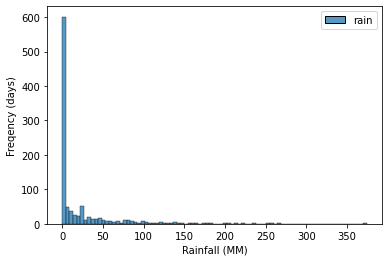
\includegraphics[width=\linewidth]{HMM_Only/0_freq_data.png}
        \caption{Observed Data}
        \label{inc0:data}
        \end{subfigure}
        \begin{subfigure}{.45\textwidth}
        \centering
        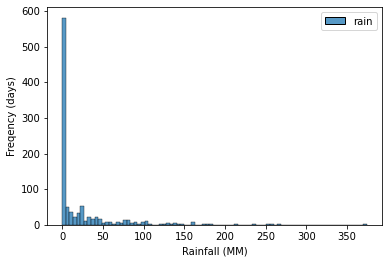
\includegraphics[width=\linewidth]{HMM_Only/0_freq_sim.png}
        \caption{Simulated Data}
        \label{inc0:sim}
        \end{subfigure}

        \begin{subfigure}{.45\textwidth}
        \centering
        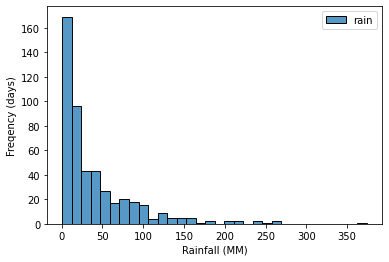
\includegraphics[width=\linewidth]{HMM_Only/_freq_data.png}
        \caption{Observed Data removing all 0mm days}
        \label{inc0:n0data}
        \end{subfigure}
        \begin{subfigure}{.45\textwidth}
        \centering
        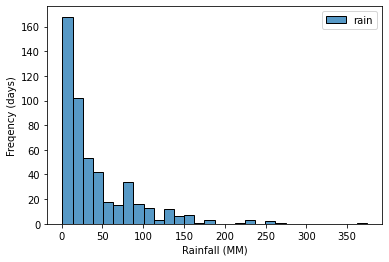
\includegraphics[width=\linewidth]{HMM_Only/_freq_sim.png}
        \caption{Simulated Data removing all 0mm days}
        \label{inc0:n0sim}
        \end{subfigure}
        \caption{Comparison of Observed data and Data simulated by HMM}
        \label{inc0}
    \end{figure}

    Figure \ref{inc0} shows that the frequencies seem to be similar for both simulations and recorded data. Furthermore, more minor details such as the peak at around 25mm also remains consistent. While this is promising, the large frequency for 0mm distorts the graph. To compare further, we plot the histograms once more, removing the first bar for 0mm. Here we can see it is not identical but seems to have similar properties, such as max, medium and high-density areas. We will investigate this result numerically in the results chapter of this paper.


    